\chapter{Силы, фазовое пространство и законы сохранения}

\lectureoverview{Закон движения должен делать больше, чем просто связывать знакомые физические величины. Он должен задавать состояние системы, переводить это состояние от одного момента к следующему и показывать, какие различия и какие величины сохраняются при движении. Мы придём к ньютоновской механике, сначала проверив правдоподобный, но неверный закон силы, затем расширив описание состояния от положения до фазового пространства и, наконец, выведя законы сохранения импульса и энергии.}

\section{Полезный неверный закон}

В повседневном движении доминирует трение. Если толкать тяжёлый предмет по полу, он движется; если перестать толкать, он вскоре останавливается. Большее усилие обычно даёт большую скорость, тогда как более тяжёлый предмет требует большего усилия. В таком мире естественно предположить, что сила порождает саму скорость. Именно на этой интуиции основывалось аристотелевское описание движения.

Катание на коньках даёт недостающий опыт. Конькобежцу нужна сила, чтобы начать движение, остановиться или изменить направление, но не для того, чтобы, начав двигаться, продолжать скользить. Если бы Аристотель имел дело с почти лишённым трения льдом, а не с обычной землёй, не заметить изъян в представлении сила--скорость было бы гораздо труднее.

Чтобы выявить, что именно неверно в этой интуиции, придадим ей точную современную форму. Запишем заведомо неверное уравнение

\begin{equation}
  \mathbf F=m\mathbf v.
  \label{eq:aristotle-vector-law}
\end{equation}

Это не закон Ньютона, и его не следует заучивать как физику. Его ценность диагностическая: как только словесное правило превращено в уравнение, можно спросить, предсказывает ли оно движение и сохраняет ли достаточно информации, чтобы восстановить прошлое. Краткое обсуждение на занятии греческого слова для силы отсылает к \emph{dynamis}, корню, который слышен также в словах динамо и динамика, но терминология вторична по сравнению с проверкой самого закона.

\begin{figure}[htbp]
  \centering
  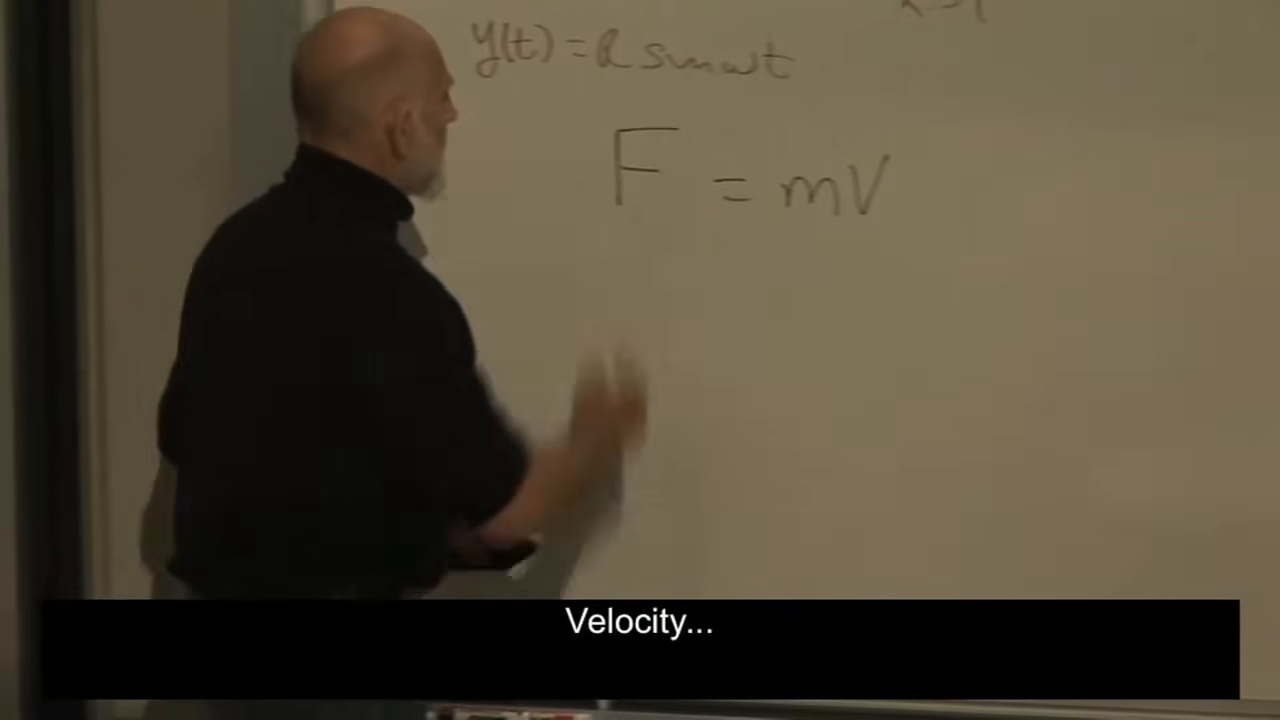
\includegraphics[width=0.82\textwidth]{lecture_02_figure_02.png}
  \caption{Намеренно неверный закон сила--скорость, используемый для проверки предсказуемости и обратимости.}
  \lectureframe{00:04:51}
\end{figure}

Ограничим движение одной пространственной координатой. Поскольку \(v=\dot x\), закон принимает вид

\begin{equation}
  F(t)=m\dot x(t).
  \label{eq:aristotle-1d}
\end{equation}

Теперь разобьём время на короткие интервалы длины \(\delta\). За один такой интервал,

\begin{equation}
  \dot x(t)\simeq
  \frac{x(t+\delta)-x(t)}{\delta}.
  \label{eq:first-difference}
\end{equation}

Подстановка в уравнение~\eqref{eq:aristotle-1d} даёт

\begin{equation}
  x(t+\delta)
  =x(t)+\frac{\delta}{m}F(t).
  \label{eq:aristotle-update}
\end{equation}

Это действительно имеет вид правила обновления. Если известны текущее положение и сила, то положение в следующий стробоскопический момент определяется однозначно. Однако когда сила исчезает, правило Аристотеля даёт \(\dot x=0\): объект должен оставаться в покое. Движение без поддерживающей силы исключается с самого начала.

\begin{figure}[htbp]
  \centering
  \includegraphics[width=0.84\textwidth]{lecture_02_figure_07.png}
  \caption{Дискретное обновление Аристотеля для случая возвращающей силы. На каждом шаге смещение умножается на множитель, немного меньший единицы.}
  \lectureframe{00:10:15}
\end{figure}

\subsection{Пружина в механике Аристотеля}

Рассмотрим частицу, прикреплённую к пружине, с положением равновесия при \(x=0\). Смещение создаёт возвращающую силу

\begin{equation}
  F(x)=-kx,
  \qquad k>0.
  \label{eq:hooke-law}
\end{equation}

Подставляя эту силу в уравнение~\eqref{eq:aristotle-update}, получаем

\begin{equation}
  x(t+\delta)
  =\left(1-\frac{k\delta}{m}\right)x(t).
  \label{eq:aristotle-spring-update}
\end{equation}

При достаточно малом \(\delta\) множитель в скобках оказывается чуть меньше единицы. Поэтому каждое обновление уменьшает смещение на одну и ту же долю:

\begin{equation}
  x_n=\left(1-\frac{k\delta}{m}\right)^n x_0.
  \label{eq:aristotle-geometric-decay}
\end{equation}

Непрерывное уравнение и его решение имеют вид

\begin{align}
  m\dot x&=-kx,
  \label{eq:aristotle-spring-continuous}\\
  x(t)&=x(0)e^{-kt/m}.
  \label{eq:aristotle-spring-solution}
\end{align}

Пружина не совершает колебаний. После освобождения из любого смещённого положения частица экспоненциально приближается к началу координат, двигаясь всё медленнее по мере приближения.

\begin{figure}[htbp]
  \centering
  \includegraphics[width=0.84\textwidth]{lecture_02_figure_08.png}
  \caption{Экспоненциальное решение уравнения пружины в механике Аристотеля. Смещение затухает, а не колеблется.}
  \lectureframe{00:12:02}
\end{figure}

Будущее предсказать легко: всякое начальное смещение приближается к одному и тому же состоянию покоя. С прошлым дело обстоит иначе. Предположим, что частица наблюдается очень близко к началу координат и лишь с конечной точностью. Она могла начинать с любого из многих различных смещений, поскольку все их экспоненциально малые остатки в конце концов попадают в один и тот же допуск измерения. При идеальной математической точности уравнение~\eqref{eq:aristotle-spring-solution} можно обратить по времени, но практические различия между историями неуклонно стираются. Поэтому этот закон подозрителен с точки зрения обратимой фундаментальной динамики.

Это не означает, что Аристотель был неразумен. Описанное им движение, в котором доминирует трение, действительно диссипативно. Ошибкой было возвести это эффективное поведение в ранг фундаментального закона. Само трение есть сила, возникающая из сложных микроскопических взаимодействий. Когда рука толкает тело с приблизительно постоянной скоростью, приложенная сила уравновешивает трение; приложенная сила как таковая не создаёт скорость.

\section{Закон Ньютона и его физический смысл}

Ньютоновская поправка состоит в том, что сила изменяет движение:

\begin{equation}
  \mathbf F=m\mathbf a=m\ddot{\mathbf x}.
  \label{eq:newton-second-law}
\end{equation}

Прежде чем рассматривать это как уравнение эволюции, надо распутать два кажущихся логических круга. Первый касается систем отсчёта. Часто говорят, что законы Ньютона выполняются в инерциальных системах отсчёта, а инерциальная система отсчёта — это такая система, в которой выполняются законы Ньютона. Физическое утверждение состоит не в этом циклическом определении. Оно состоит в эмпирическом утверждении, что \emph{существуют} системы отсчёта, задаваемые подходящими линейками и часами, в которых законы Ньютона принимают свой простой вид. В системах, ускоряющихся или вращающихся относительно них, необходимы дополнительные фиктивные силы. То, как уравнения преобразуются в этих других системах, можно выяснить позже.

Второй логический круг касается силы и массы. Если силу определить как произведение массы на ускорение, а массу — как силу, делённую на ускорение, уравнение кажется пустым. Операциональный эксперимент отделяет определения от закона. Сравните тело с эталонным килограммом, уравновесив их, а затем присоедините это тело к пружинному динамометру в пространстве, где в остальном силы отсутствуют. За одну единицу силы примем фиксированное малое удлинение пружины. Две одинаковые пружины, каждая растянутая на ту же величину, дают две единицы силы и создают вдвое большее ускорение. Добавить вторую пружину надёжнее, чем растянуть одну пружину вдвое сильнее, потому что реальная пружина в конце концов становится нелинейной или рвётся. Если оставить одну пружину, но соединить две равные массы, ускорение будет вдвое меньше; для трёх равных масс — втрое меньше.

\begin{figure}[htbp]
  \centering
  \includegraphics[width=0.84\textwidth]{lecture_02_figure_09.png}
  \caption{Мысленный эксперимент с пружинным динамометром, используемый для задания равных единиц силы и проверки пропорциональности ускорения силе.}
  \lectureframe{00:22:45}
\end{figure}

Эти сравнения придают эмпирический смысл утверждению

\begin{equation}
  a\propto F,
  \qquad
  a\propto\frac{1}{m},
  \qquad
  F=ma.
  \label{eq:force-mass-scaling}
\end{equation}

Словом \emph{particle} мы будем обозначать любой малый объект, внутренняя структура которого несущественна, а не только элементарную частицу.

\subsection{Почему одно лишь положение не задаёт состояние}

Теперь проверим уравнение Ньютона тем же стробоскопическим методом. Центрированная конечная разность для ускорения имеет вид

\begin{equation}
  \ddot x(t)\simeq
  \frac{x(t+\delta)-2x(t)+x(t-\delta)}{\delta^2}.
  \label{eq:second-difference}
\end{equation}

Таким образом, уравнение Ньютона даёт

\begin{equation}
  x(t+\delta)
  =2x(t)-x(t-\delta)+\frac{\delta^2}{m}F(t).
  \label{eq:newton-position-update}
\end{equation}

Следующее положение нельзя получить из одного лишь \(x(t)\). Нужно также знать предыдущее положение \(x(t-\delta)\) или, что эквивалентно, скорость в настоящий момент. На первый взгляд из-за этого уравнение Ньютона кажется менее предсказательным, чем правило Аристотеля. Но правильный вывод иной: одно лишь положение было неполным описанием состояния. Знать всё существенное в данный момент — значит знать достаточно данных, чтобы определить последующее движение. Для ньютоновской частицы этими данными являются положение и скорость.

\section{Импульс и фазовое пространство}

Введём импульс соотношением

\begin{equation}
  \mathbf p=m\mathbf v=m\dot{\mathbf x}.
  \label{eq:momentum-definition}
\end{equation}

Массу выбранной ньютоновской системы считают постоянной. Объект может потерять часть себя, как ручка может потерять колпачок, но тогда изменился сам описываемый объект; у выбранной замкнутой системы полная масса всё равно постоянна. При постоянной \(m\) второй закон Ньютона принимает вид

\begin{equation}
  \mathbf F=\dot{\mathbf p}.
  \label{eq:newton-momentum-form}
\end{equation}

\begin{figure}[htbp]
  \centering
  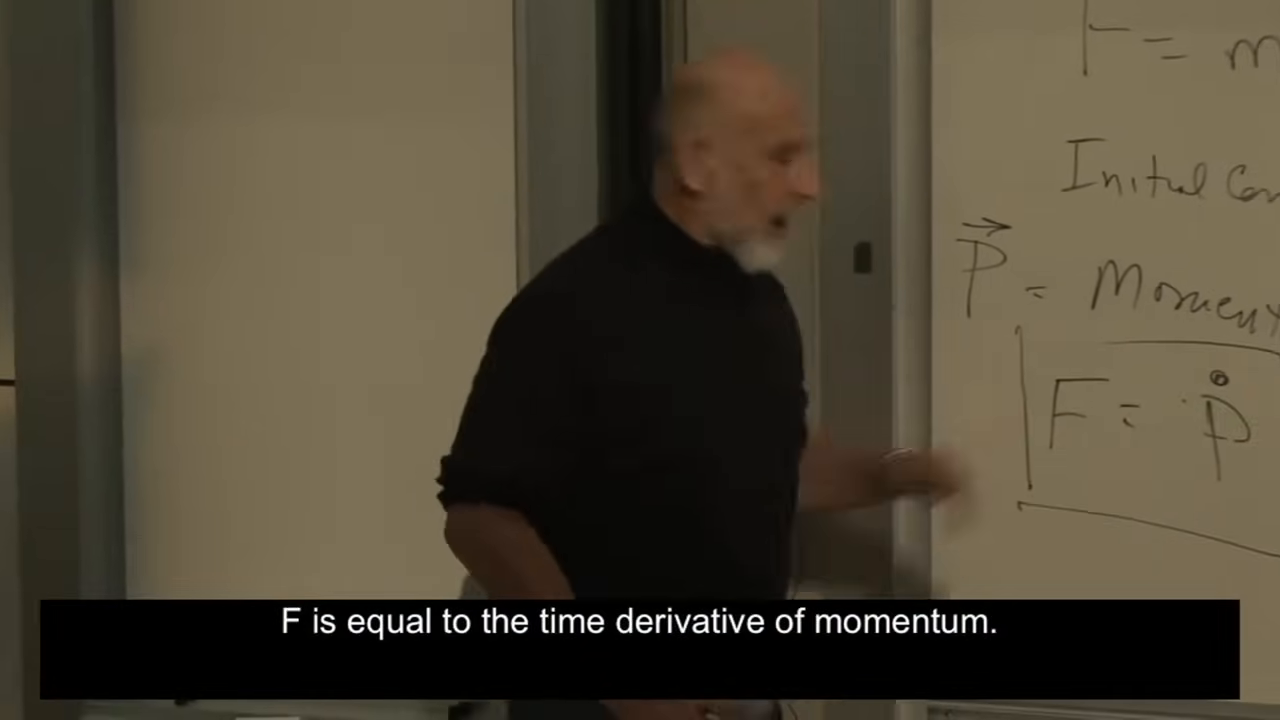
\includegraphics[width=0.82\textwidth]{lecture_02_figure_03.png}
  \caption{Закон Ньютона, записанный через производную импульса по времени.}
  \lectureframe{00:32:35}
\end{figure}

Для одной координаты ньютоновское движение теперь можно записать как два уравнения первого порядка для двух независимых переменных состояния:

\begin{align}
  \dot p&=F(x,t),
  \label{eq:first-order-p}\\
  \dot x&=\frac{p}{m}.
  \label{eq:first-order-x}
\end{align}

Одно уравнение говорит, как сила изменяет импульс; другое — как импульс изменяет положение. Их дискретная форма первого порядка имеет вид

\begin{align}
  p(t+\delta)&=p(t)+\delta F(x(t),t)+O(\delta^2),
  \label{eq:momentum-discrete}\\
  x(t+\delta)&=x(t)+\frac{\delta}{m}p(t)+O(\delta^2).
  \label{eq:position-discrete}
\end{align}

Если заданы \(x(t)\) и \(p(t)\), эти уравнения определяют следующую пару, которая затем служит входом для следующего шага. Траектория строится последовательными обновлениями.

\begin{figure}[htbp]
  \centering
  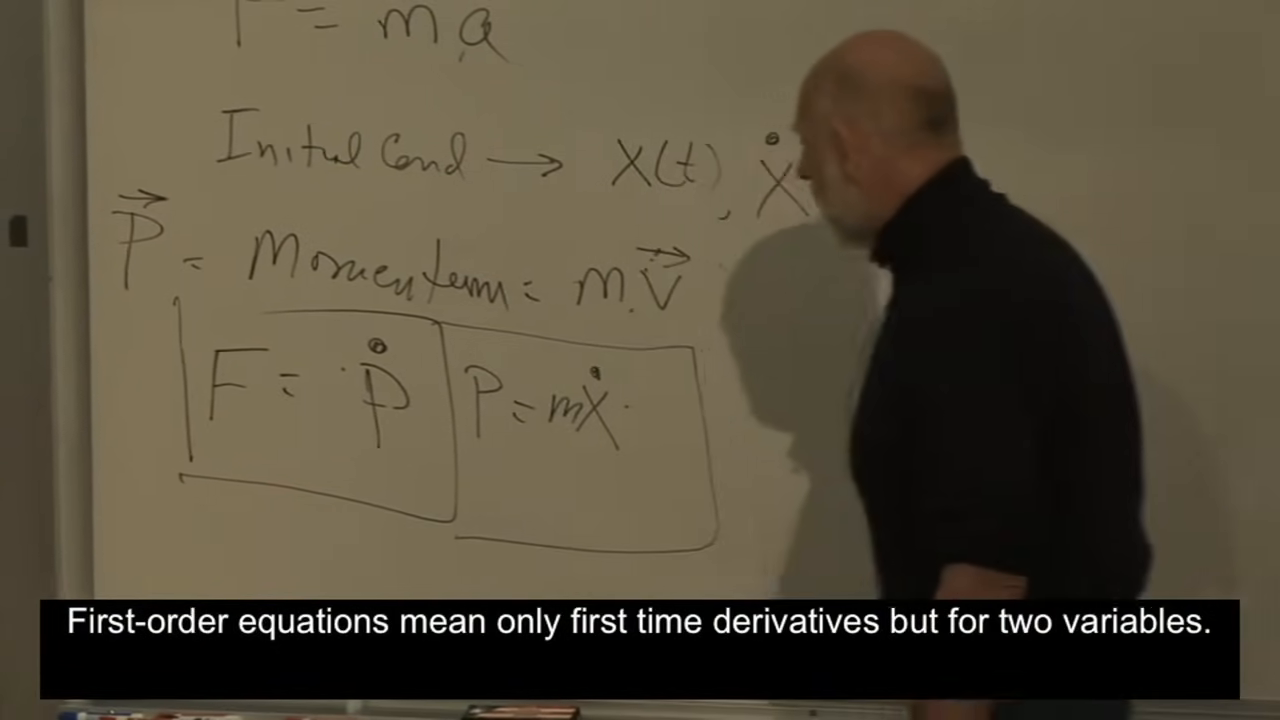
\includegraphics[width=0.84\textwidth]{lecture_02_figure_04.png}
  \caption{Два уравнения первого порядка и соответствующие начальные данные. Положение и импульс вместе задают состояние.}
  \lectureframe{00:35:47}
\end{figure}

Пространство всех пар \((x,p)\) называется \emph{фазовым пространством}. Для одной частицы, движущейся в трёх измерениях, оно имеет шесть координат,

\begin{equation}
  (x,y,z,p_x,p_y,p_z).
  \label{eq:one-particle-phase-space}
\end{equation}

Фазовое пространство — это пространство полных начальных условий. Конфигурационное пространство фиксирует только положения; фазовое пространство фиксирует в точности те данные, которые требуются закону движения.

\begin{classroomqa}
  \audiencequestion{Если сила является функцией положения, а не известной функцией времени, становится ли процедура обновления более сложной?\lecturetimestamp{00:36:27--00:37:07}}
  \lecturerresponse{Уравнения остаются предсказательными. Как только известны \(x\) и \(p\), известна и величина \(F(x)\). Уравнение~\eqref{eq:first-order-p} даёт следующее значение \(p\), уравнение~\eqref{eq:first-order-x} — \(x\), и обновлённую пару можно снова использовать.}
\end{classroomqa}

\section{Ньютоновская пружина}

Вернёмся к пружине, чтобы сравнить два закона в одних и тех же физических условиях. По Ньютону получаем

\begin{equation}
  m\ddot x=-kx.
  \label{eq:newton-spring}
\end{equation}

Временно положим \(m=k=1\), чтобы убрать константы. Тогда

\begin{equation}
  \ddot x=-x.
  \label{eq:normalized-oscillator}
\end{equation}

В отличие от экспоненты, синус либо косинус после двукратного дифференцирования возвращается к себе с противоположным знаком. Общее решение можно записать в виде

\begin{align}
  x(t)&=C\cos(t-t_0),
  \label{eq:oscillator-x}\\
  p(t)=\dot x(t)&=-C\sin(t-t_0).
  \label{eq:oscillator-p}
\end{align}

Эти две константы несут две части начальной информации. Амплитуда \(C\) задаёт максимальное смещение, тогда как \(t_0\) фиксирует фазу, выбранную здесь так, что скорость обращается в нуль при \(t=t_0\). Частица останавливается в концах лишь на мгновение. Затем она проходит обратно через начало координат, где её скорость и импульс максимальны, и продолжает колебаться.

Возводя в квадрат уравнения~\eqref{eq:oscillator-x} и \eqref{eq:oscillator-p}, получаем

\begin{equation}
  x^2+p^2=C^2.
  \label{eq:oscillator-phase-circle}
\end{equation}

Таким образом, точка фазового пространства движется по окружности радиуса \(C\). Разные начальные амплитуды дают разные окружности; изменение \(t_0\) выбирает другую начальную точку на той же окружности. Каждая окружность обходится с одним и тем же периодом \(2\pi\) в этих нормированных единицах, независимо от амплитуды.

\begin{figure}[htbp]
  \centering
  \includegraphics[width=0.84\textwidth]{lecture_02_figure_10.png}
  \caption{Решение осциллятора и его круговая орбита на фазовой плоскости \((x,p)\).}
  \lectureframe{00:43:20}
\end{figure}

\begin{figure}[htbp]
  \centering
  \begin{tikzpicture}[scale=1.05,>=Latex]
    \draw[->] (-2.6,0) -- (2.75,0) node[right] {$x$};
    \draw[->] (0,-2.4) -- (0,2.55) node[above] {$p$};
    \draw[blue!65!black,thick] (0,0) circle (1.85);
    \draw[->,blue!65!black,thick]
      (1.60,0.93) arc[start angle=30,end angle=72,radius=1.85];
    \fill[red!65!black] (1.60,0.93) circle (2pt);
    \draw[dashed] (0,0) -- (1.60,0.93)
      node[midway,below right] {$C$};
    \node[align=left] at (-1.55,1.85)
      {$x=C\cos(t-t_0)$\\$p=-C\sin(t-t_0)$};
  \end{tikzpicture}
  \caption{Орбита в фазовом пространстве сохраняет информацию и о положении, и об импульсе. Её радиус характеризует движение, тогда как угол равномерно растёт со временем.}
  \label{fig:oscillator-phase-space}
\end{figure}

Проекция на горизонтальную ось даёт привычное возвратно-поступательное движение \(x\); проекция на вертикальную ось даёт колебание \(p\). В отличие от аристотелевой пружины, разные окружности никогда не сливаются друг с другом. Знание точки фазового пространства определяет и её будущее, и её прошлое.

Для произвольных \(m\) и \(k\) угловая частота равна

\begin{equation}
  \omega=\sqrt{\frac{k}{m}},
  \qquad
  x(t)=C\cos\bigl(\omega(t-t_0)\bigr),
  \label{eq:general-oscillator-frequency}
\end{equation}

и фазовая орбита становится эллипсом на ненормированной плоскости \((x,p)\). Картина с окружностью соответствует удобной нормировке \(m=k=1\), использованной в лекции.

\begin{classroomqa}
  \audiencequestion{Если бы вторую производную в уравнении осциллятора заменить первой, исчезла бы предсказуемость?\lecturetimestamp{00:45:23--00:46:04}}
  \lecturerresponse{Нет. Уравнение первого порядка всё ещё может предсказывать дальнейшее движение по подходящим начальным данным. Более серьёзный вопрос состоит в том, сохраняет ли порождаемый им поток различия достаточно хорошо, чтобы быть обратимым; соответствующая общая теорема отложена до тех пор, пока не будет введён необходимый аппарат.}
\end{classroomqa}

\section{Обращение времени}

Картина с осциллятором делает обратимость наглядной, но есть и непосредственная проверка на уровне уравнений. Введём обращённую временную координату

\begin{equation}
  T=-t.
  \label{eq:reverse-time}
\end{equation}

Тогда

\begin{equation}
  \frac{d}{dt}=-\frac{d}{dT},
  \qquad
  \frac{d^2}{dt^2}=\frac{d^2}{dT^2}.
  \label{eq:time-derivative-parity}
\end{equation}

Первая производная при обращении времени меняет знак, тогда как вторая — нет. Следовательно, автономное аристотелево уравнение

\begin{equation}
  m\dot x=F(x)
  \label{eq:aristotle-time-reversal}
\end{equation}

не сохраняет своей формы, если прокрутить фильм назад. Затухающая пружина превратилась бы в пружину, которая самопроизвольно уходит от равновесия. Напротив,

\begin{equation}
  m\ddot x=F(x)
  \label{eq:newton-time-reversal}
\end{equation}

не изменяется. При обращении ньютоновского фильма скорость меняет знак, а ускорение остаётся неизменным, так что фильм, прокрученный назад, — это ещё одно допустимое решение.

\begin{figure}[htbp]
  \centering
  \includegraphics[width=0.84\textwidth]{lecture_02_figure_11.png}
  \caption{Сравнение на доске при \(t\mapsto -t\): первые производные меняют знак, тогда как вторые — нет.}
  \lectureframe{00:50:45}
\end{figure}

\begin{classroomqa}
  \audiencequestion{Почему обратимость следует принимать как посылку о физике вообще?\lecturetimestamp{00:46:16--00:48:26}}
  \lecturerresponse{Её проверяют, а не гарантируют определением. Мы рассматриваем успешные законы, выявляем общие экспериментальные особенности и возводим эти особенности в ранг принципов. Более глубокий логический порядок обратный: квантовая теория поля фундаментальнее, а ньютоновская механика возникает через приближения, такие как малые скорости и тяжёлые объекты. Курс должен строиться снизу вверх, начиная с более простых законов, поэтому обратимость вводится сейчас как принцип, область применимости которого будет проверена позже.}
\end{classroomqa}

\begin{classroomqa}
  \audiencequestion{Была ли сама обратимость вопросом, который Ньютон сознательно ставил?\lecturetimestamp{00:48:28--00:49:02}}
  \lecturerresponse{Исторический ответ неопределён. Ньютон, несомненно, понимал инерцию: сила нужна, чтобы изменить состояние движения, а не для поддержания равномерного движения. Оформлял ли он это понимание явно в терминах обратимости — отдельный исторический вопрос.}
\end{classroomqa}

\section{Циклы и сохраняющиеся величины}

Окружности в фазовом пространстве подсказывают следующую идею. Траектория остаётся на одной окружности и никогда не перескакивает на другую. Поэтому каждой окружности можно сопоставить число, которое остаётся постоянным в ходе движения. Для нормированного осциллятора это число равно

\begin{equation}
  C^2=x^2+p^2.
  \label{eq:cycle-label}
\end{equation}

С точностью до множителя одна вторая это энергия осциллятора. Большим окружностям соответствует большая энергия; изменение начальной фазы её не меняет. Мы выведем это утверждение, а не просто прочитаем его с рисунка, но сначала рассмотрим импульс.

Первый закон Ньютона утверждает, что тело, на которое не действует суммарная сила, движется с постоянной скоростью. Он уже содержится во втором законе:

\begin{equation}
  \mathbf F=0
  \quad\Longrightarrow\quad
  \dot{\mathbf p}=0
  \quad\Longrightarrow\quad
  \mathbf v=\text{constant}
  \label{eq:newton-first-from-second}
\end{equation}

при постоянной массе. Третий закон Ньютона вносит действительно новую информацию о взаимодействиях между частицами.

\subsection{Равные, противоположные и центральные силы}

Пусть \(\mathbf F_{ij}\) обозначает силу, действующую на частицу \(i\) со стороны частицы \(j\). Тогда часть третьего закона, утверждающая равенство по величине и противоположность по направлению, имеет вид

\begin{equation}
  \mathbf F_{ij}=-\mathbf F_{ji}.
  \label{eq:newton-third-pair}
\end{equation}

Если бы две силы были направлены в одну и ту же сторону, изолированная пара могла бы самопроизвольно ускоряться. Это была бы машина без рабочего тела, создающая движение только за счет внутренних сил. Такого поведения не наблюдается.

\begin{figure}[htbp]
  \centering
  \includegraphics[width=0.84\textwidth]{lecture_02_figure_12.png}
  \caption{Индексная запись утверждения о равенстве по величине и противоположности сил взаимодействия.}
  \lectureframe{00:59:25}
\end{figure}

Для рассматриваемых здесь сил между точечными частицами обе силы пары, кроме того, направлены вдоль прямой, соединяющей центры частиц. Равные по величине и противоположно направленные силы, не лежащие на одной прямой, могли бы образовать чистый крутящий момент и привести изолированную жесткую пару во вращение. Условие центральной силы исключает эту возможность:

\begin{equation}
  \mathbf F_{ij}\parallel
  (\mathbf r_i-\mathbf r_j).
  \label{eq:central-force-condition}
\end{equation}

Условие равенства и противоположности приводит к сохранению импульса. Условие линии центров связано с законом сохранения момента импульса, который будет изучаться позже.

\begin{figure}[htbp]
  \centering
  \includegraphics[width=0.84\textwidth]{lecture_02_figure_13.png}
  \caption{Центрально-силовая часть третьего закона Ньютона: силы взаимодействия лежат на прямой, соединяющей частицы.}
  \lectureframe{01:01:38}
\end{figure}

\subsection{Полный импульс}

Рассмотрим замкнутую систему из \(N\) частиц. Внешних сил нет; единственные силы — это силы взаимодействия частиц друг с другом. Аддитивность сил и второй закон Ньютона дают для каждой частицы

\begin{equation}
  \dot{\mathbf p}_i
  =m_i\ddot{\mathbf r}_i
  =\sum_{\substack{j=1\\j\ne i}}^N \mathbf F_{ij}.
  \label{eq:many-particle-newton}
\end{equation}

Просуммируем это уравнение по \(i\):

\begin{align}
  \frac{d}{dt}\sum_{i=1}^N\mathbf p_i
  &=\sum_{i=1}^N
    \sum_{\substack{j=1\\j\ne i}}^N\mathbf F_{ij}
  \notag\\
  &=\sum_{i<j}\bigl(\mathbf F_{ij}+\mathbf F_{ji}\bigr)
  =0.
  \label{eq:momentum-pair-cancellation}
\end{align}

Каждое взаимодействие появляется дважды, по одному разу в каждом направлении, и члены пары сокращаются. Введя обозначение

\begin{equation}
  \mathbf P_{\mathrm{tot}}=\sum_{i=1}^N\mathbf p_i,
  \label{eq:total-momentum}
\end{equation}

получаем первый закон сохранения:

\begin{equation}
  \frac{d\mathbf P_{\mathrm{tot}}}{dt}=0.
  \label{eq:momentum-conservation}
\end{equation}

\begin{figure}[htbp]
  \centering
  \includegraphics[width=0.84\textwidth]{lecture_02_figure_14.png}
  \caption{Суммирование уравнений для частиц приводит к сокращению попарных сил, так что производная полного импульса равна нулю.}
  \lectureframe{01:04:38}
\end{figure}

Исторически мы представили сохранение импульса как следствие третьего закона Ньютона. В современной физике сохранение импульса часто рассматривается как более фундаментальное утверждение: если в изолированной двухчастичной системе сохраняется полный импульс, то изменения импульсов ее частиц должны быть равны по величине и противоположны по направлению. Однако для данного изложения полезен именно ньютоновский путь.

\section{Энергия в одном измерении}

Рассмотрим частицу, движущуюся вдоль прямой под действием силы, зависящей только от ее положения:

\begin{equation}
  F=F(x).
  \label{eq:position-force}
\end{equation}

Такая сила называется не зависящей от времени. Это не означает, что сила, действующая на движущуюся частицу, имеет постоянное численное значение. Ее значение меняется по мере изменения \(x(t)\). Это означает, что всякий раз, когда частица находится в одном и том же положении \(x\), на нее действует одна и та же сила, независимо от момента времени.

В одном измерении любую достаточно регулярную функцию силы можно проинтегрировать. Поэтому потенциальную энергию \(V(x)\) определим соотношением

\begin{equation}
  F(x)=-\frac{dV}{dx},
  \label{eq:potential-definition-1d}
\end{equation}

или, что эквивалентно,

\begin{equation}
  V(x)=-\int^x F(u)\,du+V_0.
  \label{eq:potential-integral}
\end{equation}

Аддитивная постоянная \(V_0\) не влияет на силу. Представьте \(V(x)\) как высоту ландшафта над осью \(x\). Частица подталкивается в сторону меньшей высоты, и сила больше там, где наклон круче. В верхней или нижней точке гладкого холма наклон обращается в нуль, так что там сила равна нулю.

\begin{figure}[htbp]
  \centering
  \includegraphics[width=0.84\textwidth]{lecture_02_figure_15.png}
  \caption{Потенциальная энергия как одномерный ландшафт. Сила направлена вниз по склону, а ее величина определяется наклоном.}
  \lectureframe{01:12:57}
\end{figure}

Определим кинетическую, потенциальную и полную энергию соотношениями

\begin{equation}
  T=\frac12m\dot x^2,
  \qquad
  E=T+V(x)
  =\frac12m\dot x^2+V(x).
  \label{eq:energy-1d}
\end{equation}

На данном этапе энергия — это просто название, присвоенное этой предполагаемой сохраняющейся величине. Ее физическую интерпретацию подсказывает картина ландшафта: движение вниз по склону уменьшает \(V\), одновременно увеличивая скорость и, следовательно, \(T\); движение вверх по склону делает обратное. Уравнение Ньютона доказывает, что этот обмен является точным.

Продифференцируем уравнение ~\eqref{eq:energy-1d}. Поскольку \(m\) — постоянная, а \(V\) зависит от времени только через \(x(t)\),

\begin{align}
  \frac{dE}{dt}
  &=m\dot x\ddot x+\frac{dV}{dx}\dot x
  \notag\\
  &=\dot x\left(m\ddot x+\frac{dV}{dx}\right).
  \label{eq:energy-derivative-1d}
\end{align}

Закон Ньютона и определение \(V\) дают

\begin{equation}
  m\ddot x=F=-\frac{dV}{dx}.
  \label{eq:newton-potential-1d}
\end{equation}

Следовательно, выражение в скобках в уравнении ~\eqref{eq:energy-derivative-1d} обращается в нуль:

\begin{equation}
  \frac{dE}{dt}=0.
  \label{eq:energy-conservation-1d}
\end{equation}

\begin{figure}[htbp]
  \centering
  \includegraphics[width=0.84\textwidth]{lecture_02_figure_16.png}
  \caption{Производная энергии в одномерном случае разлагается на множитель скорости и уравнение Ньютона.}
  \lectureframe{01:19:18}
\end{figure}

В одном измерении не потребовалось никакого дополнительного динамического предположения сверх регулярной силы, зависящей от положения, поскольку любая такая сила имеет первообразную.

\section{Несколько измерений и консервативные силы}

Для частицы с координатами \(x_i\) уравнение Ньютона по компонентам имеет вид

\begin{equation}
  F_i(\mathbf x)=m\ddot x_i.
  \label{eq:newton-components}
\end{equation}

Компонента силы \(F_i\) может зависеть от всех координат, а не только от \(x_i\). Мы хотели бы найти одну скалярную функцию \(V(\mathbf x)\) такую, что

\begin{equation}
  F_i(\mathbf x)
  =-\frac{\partial V(\mathbf x)}{\partial x_i},
  \qquad
  \mathbf F=-\boldsymbol\nabla V.
  \label{eq:gradient-force}
\end{equation}

В отличие от одномерного построения, здесь это не происходит автоматически. Три произвольные функции \(F_1,F_2,F_3\), вообще говоря, содержат больше независимой информации, чем производные одной скалярной функции. Эквивалентно, потенциал существует только тогда, когда силовое поле удовлетворяет условиям совместности, например равенству соответствующих смешанных частных производных; в односвязной области это выражается условием \(\boldsymbol\nabla\times\mathbf F=0\). Поэтому уравнение ~\eqref{eq:gradient-force} мы принимаем как физический постулат для рассматриваемого класса сил, а не как математическое тождество.

\begin{figure}[htbp]
  \centering
  \includegraphics[width=0.84\textwidth]{lecture_02_figure_17.png}
  \caption{Многомерный закон силы и контурный эскиз потенциала. Сила направлена поперек линий уровня в сторону убывания \(V\).}
  \lectureframe{01:24:15}
\end{figure}

На контурной карте \(V\) постоянно вдоль каждой линии уровня. Градиент перпендикулярен этим кривым и направлен в сторону наискорейшего возрастания; сила \(-\boldsymbol\nabla V\) направлена в сторону наискорейшего убывания.

\begin{figure}[htbp]
  \centering
  \begin{tikzpicture}[scale=1.0,>=Latex]
    \draw[->] (-3.0,0) -- (3.1,0) node[right] {$x_1$};
    \draw[->] (0,-2.4) -- (0,2.55) node[above] {$x_2$};
    \draw[orange!65!black,thick]
      plot[smooth cycle] coordinates
      {(-0.55,-0.35) (0.15,-0.55) (0.72,-0.10) (0.50,0.53) (-0.25,0.65)};
    \draw[orange!65!black,thick]
      plot[smooth cycle] coordinates
      {(-1.15,-0.75) (0.20,-1.10) (1.35,-0.25) (1.10,0.95) (-0.45,1.25)};
    \draw[orange!65!black,thick]
      plot[smooth cycle] coordinates
      {(-1.85,-1.20) (0.15,-1.70) (2.15,-0.40) (1.70,1.50) (-0.80,1.85)};
    \draw[->,blue!65!black,very thick] (1.62,0.73) -- (0.82,0.20)
      node[midway,above left] {$\mathbf F$};
    \draw[dashed,->,red!65!black,thick] (0.82,0.20) -- (1.62,0.73)
      node[midway,below right] {$\boldsymbol\nabla V$};
    \node[orange!65!black] at (-1.62,1.45) {$V=V_3$};
    \node[orange!65!black] at (-0.92,0.92) {$V=V_2$};
    \node[orange!65!black] at (-0.35,0.30) {$V=V_1$};
  \end{tikzpicture}
  \caption{Линии уровня скалярного потенциала. Градиент нормален к контурам, а консервативная сила направлена в противоположную сторону.}
  \label{fig:potential-contours}
\end{figure}

Когда выполняется уравнение ~\eqref{eq:gradient-force}, определим

\begin{equation}
  E=\frac12m\sum_i\dot x_i^2+V(x_1,\ldots,x_n).
  \label{eq:energy-many-coordinates}
\end{equation}

Кинетический член равен половине массы, умноженной на квадрат длины вектора скорости. Дифференцируя и применяя правило цепочки для функций многих переменных, получаем

\begin{align}
  \frac{dE}{dt}
  &=m\sum_i\dot x_i\ddot x_i
    +\sum_i\frac{\partial V}{\partial x_i}\dot x_i
  \notag\\
  &=\sum_i\dot x_i
    \left(m\ddot x_i+\frac{\partial V}{\partial x_i}\right)
  =0.
  \label{eq:energy-derivative-multidimensional}
\end{align}

Доказательство в точности совпадает с одномерным доказательством, снабжённым индексом, но его предпосылка сильнее: все компоненты силы должны происходить из одного потенциала.

\begin{figure}[htbp]
  \centering
  \includegraphics[width=0.84\textwidth]{lecture_02_figure_18.png}
  \caption{Производная энергии с индексом.  Каждая скобка обращается в нуль в силу соответствующей компоненты уравнения Ньютона.}
  \lectureframe{01:28:30}
\end{figure}

Для \(N\) частиц в трёх измерениях соберём все координаты в один список

\begin{equation}
  \begin{aligned}
    q_a={}&(x_1,y_1,z_1,x_2,y_2,z_2,\ldots,\\[-0.2em]
           &\phantom{(}x_N,y_N,z_N),\\
    &a=1,\ldots,3N.
  \end{aligned}
  \label{eq:flattened-coordinates}
\end{equation}

Имеется \(3N\) координатных компонент, но только \(N\) масс частиц; одна и та же масса повторяется в трёх записях, относящихся к данной частице.  Если

\begin{equation}
  F_a=-\frac{\partial V(q_1,\ldots,q_{3N})}{\partial q_a},
  \label{eq:many-particle-conservative-force}
\end{equation}

тогда

\begin{equation}
  E=\sum_{A=1}^{N}\frac12m_A\lvert\dot{\mathbf r}_A\rvert^2
    +V(\mathbf r_1,\ldots,\mathbf r_N)
  \label{eq:many-particle-energy}
\end{equation}

сохраняется в силу того же вычисления.  Силы, возникающие из потенциала, называются \emph{консервативными} именно потому, что они обеспечивают этот закон сохранения; это прилагательное не имеет политического смысла.

\section{Осциллятор как контур энергии}
\enlargethispage{3\baselineskip}

Для силы пружины \(F=-kx\) уравнение~\eqref{eq:potential-definition-1d} даёт

\begin{equation}
  V(x)=\frac12kx^2+V_0.
  \label{eq:spring-potential}
\end{equation}

При выборе \(V_0=0\) энергия осциллятора равна

\begin{equation}
  E=\frac12m\dot x^2+\frac12kx^2
   =\frac{p^2}{2m}+\frac12kx^2.
  \label{eq:oscillator-energy}
\end{equation}

При \(m=k=1\),

\begin{equation}
  2E=p^2+x^2=C^2.
  \label{eq:oscillator-energy-circle}
\end{equation}

Следовательно, найденные ранее окружности в фазовом пространстве являются контурами постоянной энергии.  Для более общего одномерного потенциала эти контуры не обязаны быть окружностями, но движение всё равно происходит по кривым

\begin{equation}
  \frac{p^2}{2m}+V(x)=E
  \label{eq:general-energy-contour}
\end{equation}

на плоскости \((x,p)\).  Это возвращает нас к идее первой лекции: когда траектории остаются на различных циклах или орбитах, их может обозначать некоторое число, остающееся неизменным на протяжении всего движения.

Теперь у нас есть пространство состояний, ньютоновские уравнения эволюции и первые два закона сохранения.  Следующая формулировка механики начнётся с принципа наименьшего действия и приведёт к лагранжианам, гамильтонианам, моменту импульса и более общей структуре, стоящей за этими примерами.

\begin{classroomqa}
  \audiencequestion{Насколько точно раздаточный материал соответствует тому, что пишется на доске, и где рисунки?\lecturetimestamp{01:37:56--01:38:54}}
  \lecturerresponse{Раздаточный материал должен близко следовать лекции; если в нём отсутствует материал с доски, возможно, был отправлен не тот файл.  Рисунки ещё не были подготовлены; они появятся, шутит он, когда Continuing Studies выплатит следующий чек.}
\end{classroomqa}